\chapter{Fundamentação teórica}

Nesta Seção serão apresentadas as diferentes tecnologias disponíveis para resolver cada parte do projeto, seguidas de uma tabela comparativa das principais características, e a escolha justificada. Todas as figuras e tabelas devem ser referenciadas no texto antes de aparecer no documento. A Seção \ref{sec:exemplo} mostra um exemplo resumido do que deve ser feito para cada sensor, módulo, material, etc.

\section{Exemplo de análise de tecnologia - Comunicação sem Fio}
\label{sec:exemplo}
Como mostrado na Seção \ref{sec:objespecif}, o projeto proposto necessita de um módulo de comunicação sem fio para interagir com o aplicativo no celular do usuário. Foram analisadas as tecnologias Wi-Fi e Bluetooth, visto que estas estão presentes em praticamente todos os \textit{smartphones} modernos.

\subsection{Wi-Fi}
\label{sec:wifi}

A tecnologia Wi-Fi é tecnologia de rede sem fio criada em 1998 pela Wi-Fi Alliance, baseada no padrão IEEE 802.11. Ela é hoje a tecnologia mais comum para conexão sem fio de dispositivos à internet em dispositivos pessoais \cite{WiFi2020}. Um dos módulos mais comuns para aplicações de \sigla{IoT}{Internet of Things} (Internet das Coisas) é o ESP8266 \cite{datasheet8266}, que tem baixo custo e fácil disponibilidade de compra. Este módulo é mostrado na Figura \ref{fig:esp8266}.

\begin{figure}[!htb]
	\centering
	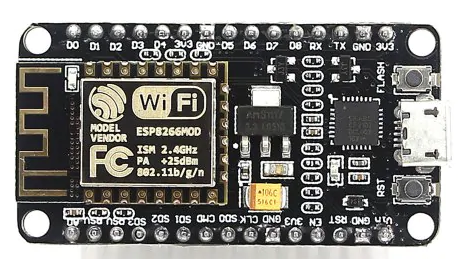
\includegraphics[width=0.4\textwidth]{./esp8266.png} 
	\caption{Foto do módulo Wi-Fi ESP8266.}
	\label{fig:esp8266}
\end{figure}

\subsection{Bluetooth}
\label{sec:bt}
A tecnologia Bluetooth foi criada em 1989, com o objetivo de substituir o protocolo RS-232 na comunicação de curta distância entre objetos fixos (citar referência). O módulo mais comum para IoT é o HC-05, mostrado na Figura \ref{fig:hc05}.

\begin{figure}[!htb]
	\centering
	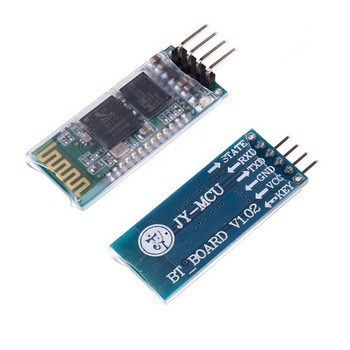
\includegraphics[width=0.4\textwidth]{./hc05.jpg} 
	\caption{Foto do módulo Bluetooth HC-05.}
	\label{fig:hc05}
\end{figure}

\subsection{Comparativo entre tecnologias de comunicação sem fio}
Na Tabela \ref{tab:semfio} são comparadas as principais características dos módulos ESP8266 e HC-05. Esta tabela foi criada com o auxílio do site \url{www.tablesgenerator.com}.

\begin{table}[!htb]
\centering
\begin{tabular}{l|l|l}
    ~       & ESP8266   & HC-05      \\
    \hline
    Alcance & 50m       & 10m        \\
    \hline
    Consumo & 170mA     & 40mA       \\
    \hline
    Preço   & R\$ 22,90 & R\$ 25,90  \\
    \hline
\end{tabular}
\caption{Comparativo entre módulos ESP8266 e HC-05}
\label{tab:semfio}
\end{table}

O módulo ESP8266 tem maior alcance e menor custo que o HC-05, como pode ser visto na Tabela \ref{tab:semfio}. Porém, como o projeto proposto será alimentado por bateria, é essencial diminuir o consumo de corrente do sistema. Por isso, foi escolhido o módulo HC-05. Além disso, o desenvolvimento de aplicações com comunicação Bluetooth já é dominado pela equipe, reduzindo a dificuldade da implementação.



